%%%%%%%%%%%%%%%%%%%%%%%%%%%%%%%%%%%%%%%%%%%%%%%%%%%%%%%%%%
\begin{frame}
  \begin{beamerboxesrounded}{}
	\begin{center}

\vspace{20pt}

		Key Design

\vspace{20pt}

	\end{center}    
  \end{beamerboxesrounded}
\end{frame}


%%%%%%%%%%%%%%%%%%%%%%%%%%%%%%%%%%%%%%%%%%%%%%%%%%%%%%%%%%
\subsection{Concepts}
%%%%%%%%%%%%%%%%%%%%%%%%%%%%%%%%%%%%%%%%%%%%%%%%%%%%%%%%%%
\frame {\frametitle{Concepts}
  \begin{itemize}
  \item \textbf{HBase has two fundamental key structures}
    \begin{itemize}
    \item Row key
    \item Column key
    \end{itemize}

    \vspace{20pt}

  \item \textbf{Both can be used to convey meaning}
    \begin{itemize}
    \item Because they store particularly meaningful data
    \item Because their sorting order is important
    \end{itemize}
  \end{itemize}
}

\frame {\frametitle{Concepts}
  \begin{itemize}
  \item \textbf{Logical vs. on-disk layout of a table}
    \begin{itemize}
    \item Main unit of separation within a table is the \textit{column
        family}
    \item The actual columns (as opposed to other column-oriented DB)
      are not used to separate data
    \item Although cells are stored logically in a table format, rows
      are stored as linear sets of the cells
    \item Cells contain all the vital information inside them
    \end{itemize}
  \end{itemize}

  \begin{figure}[h]
    \centering
    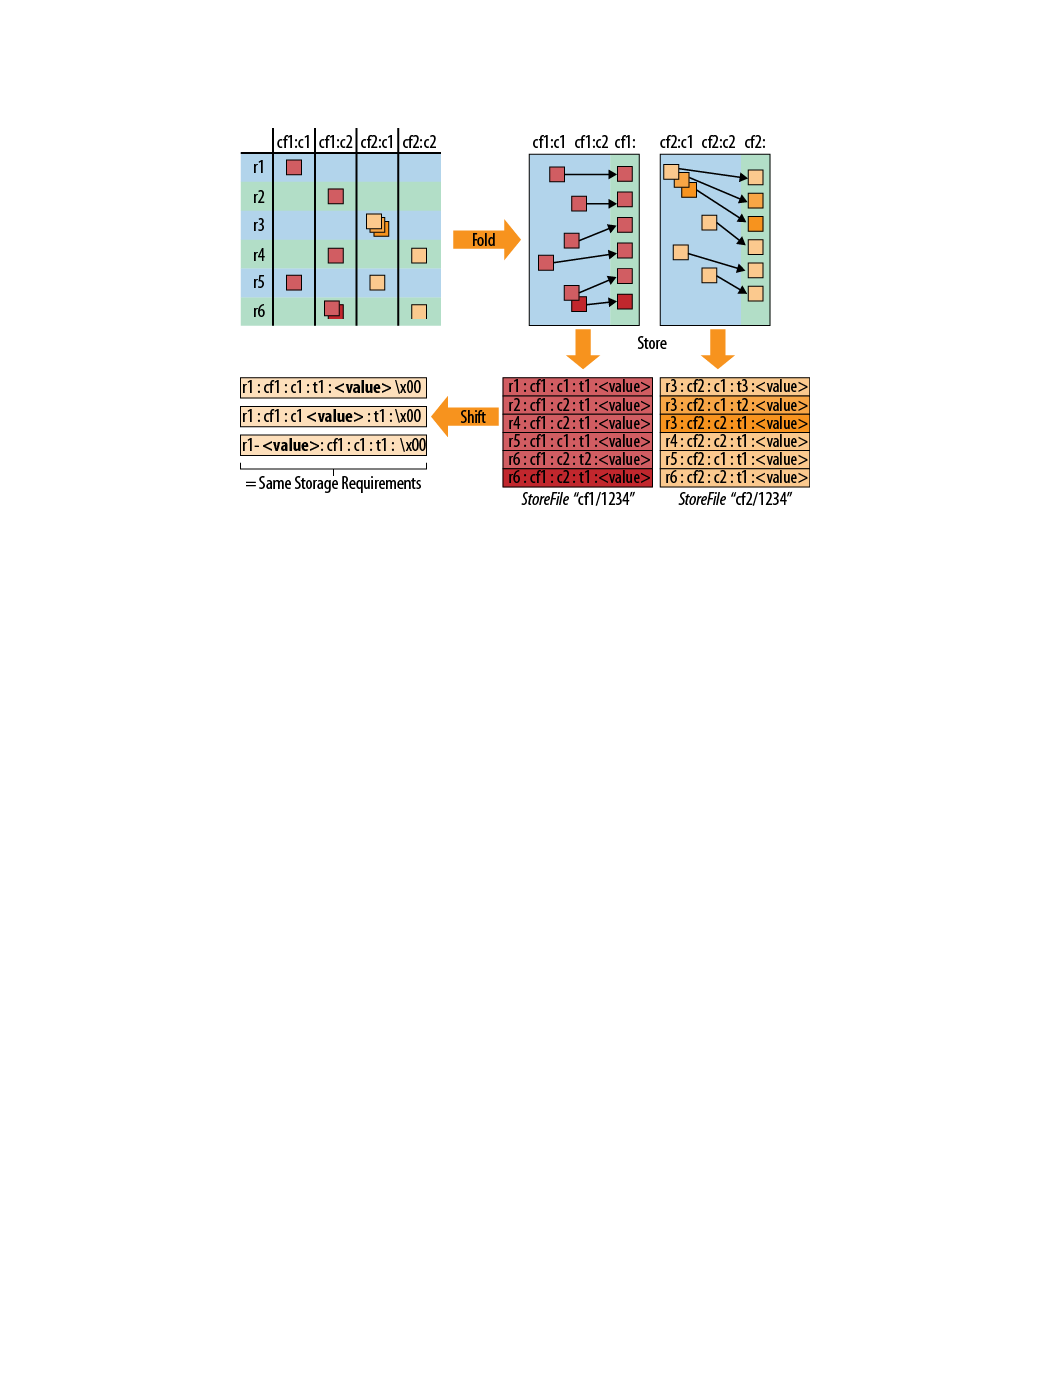
\includegraphics[scale=0.7]{./figures/layout}
  \end{figure}
}

\frame {\frametitle{Concepts}
  \begin{figure}[h]
    \centering
    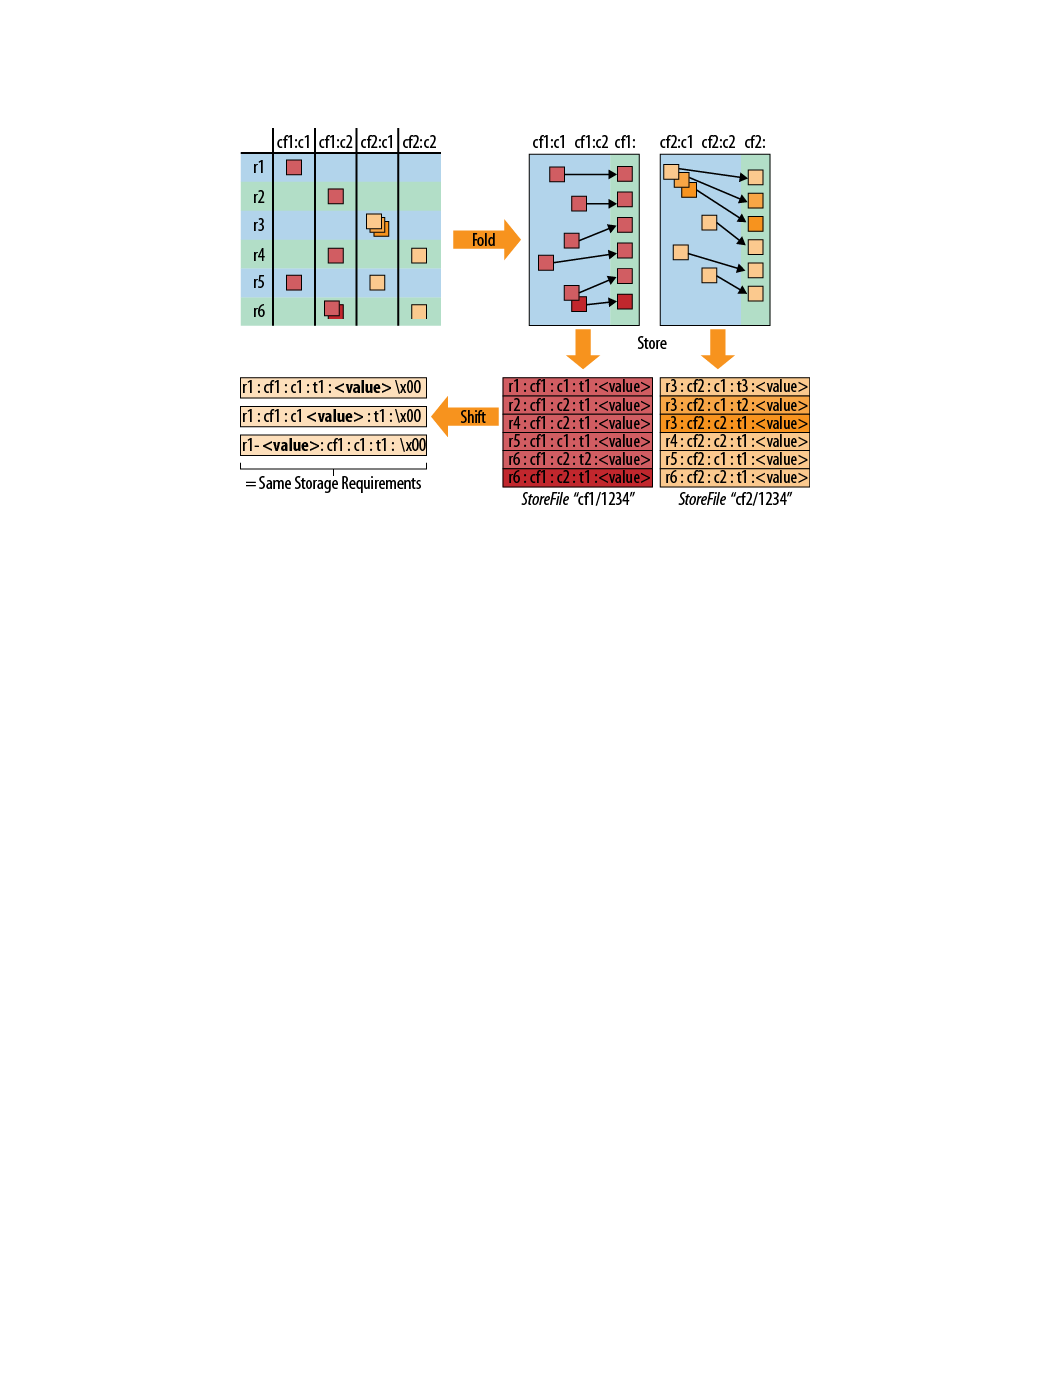
\includegraphics[scale=0.7]{./figures/layout}
  \end{figure}

  \begin{itemize}
  \item \textbf{Logical Layout (Top-Left)}
    \begin{itemize}
    \item Table consists of rows and columns
    \item Columns are the combination of a column family name and a
      column qualifier
    \item[$\to$] \texttt{<cf name: qualifier>} is the \textbf{column
        key}
    \item Rows have a \textbf{row key} to address all columns of a
      single logical row
    \end{itemize}
  \end{itemize}
}

\frame {\frametitle{Concepts}
  \begin{figure}[h]
    \centering
    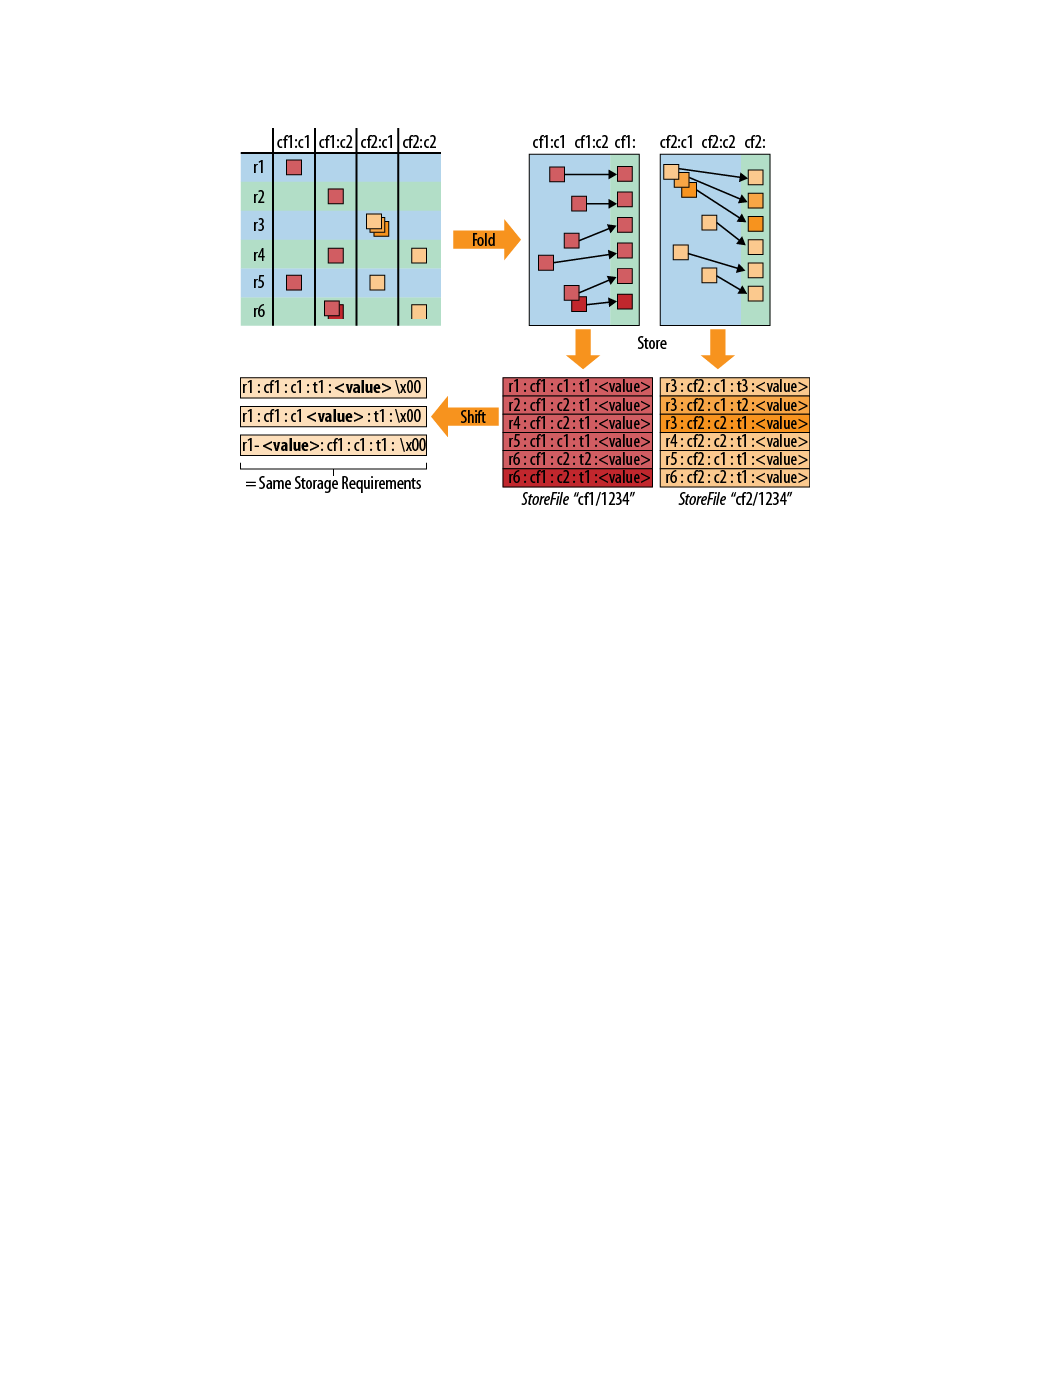
\includegraphics[scale=0.7]{./figures/layout}
  \end{figure}

  \begin{itemize}
  \item \textbf{Folding the Logical Layout (Top-Right)}
    \begin{itemize}
    \item The cells of each row are stored one after the other
    \item Each column family are stored separately
    \item[$\to$] On disk all cells of one family reside on an
      individual \texttt{StoreFile}
    \item HBase does not store unset cells
    \item[$\to$] \textbf{Row and column key is required to address every cell}
    \end{itemize}
  \end{itemize}
}

\frame {\frametitle{Concepts}
  \begin{itemize}
  \item \textbf{Versioning}
    \begin{itemize}
    \item Multiple versions of the same cell stored
      consecutively, together with the \textit{timestamp}
    \item Cells are sorted in descending order of timestamp
    \item[$\to$] Newest value first
    \end{itemize}

    \vspace{20pt}

  \item \textbf{\texttt{KeyValue} object}
    \begin{itemize}
    \item The entire cell, with all the structural information, is a
      \texttt{KeyValue} object
    \item Contains: \texttt{row key}, \texttt{<column family:
        qualifier>} $\to$ \texttt{column key}, \texttt{timestamp} and
      \texttt{value}
    \item Sorted by row key first, then by column key
    \end{itemize}

  \end{itemize}
}

\frame {\frametitle{Concepts}
  \begin{figure}[h]
    \centering
    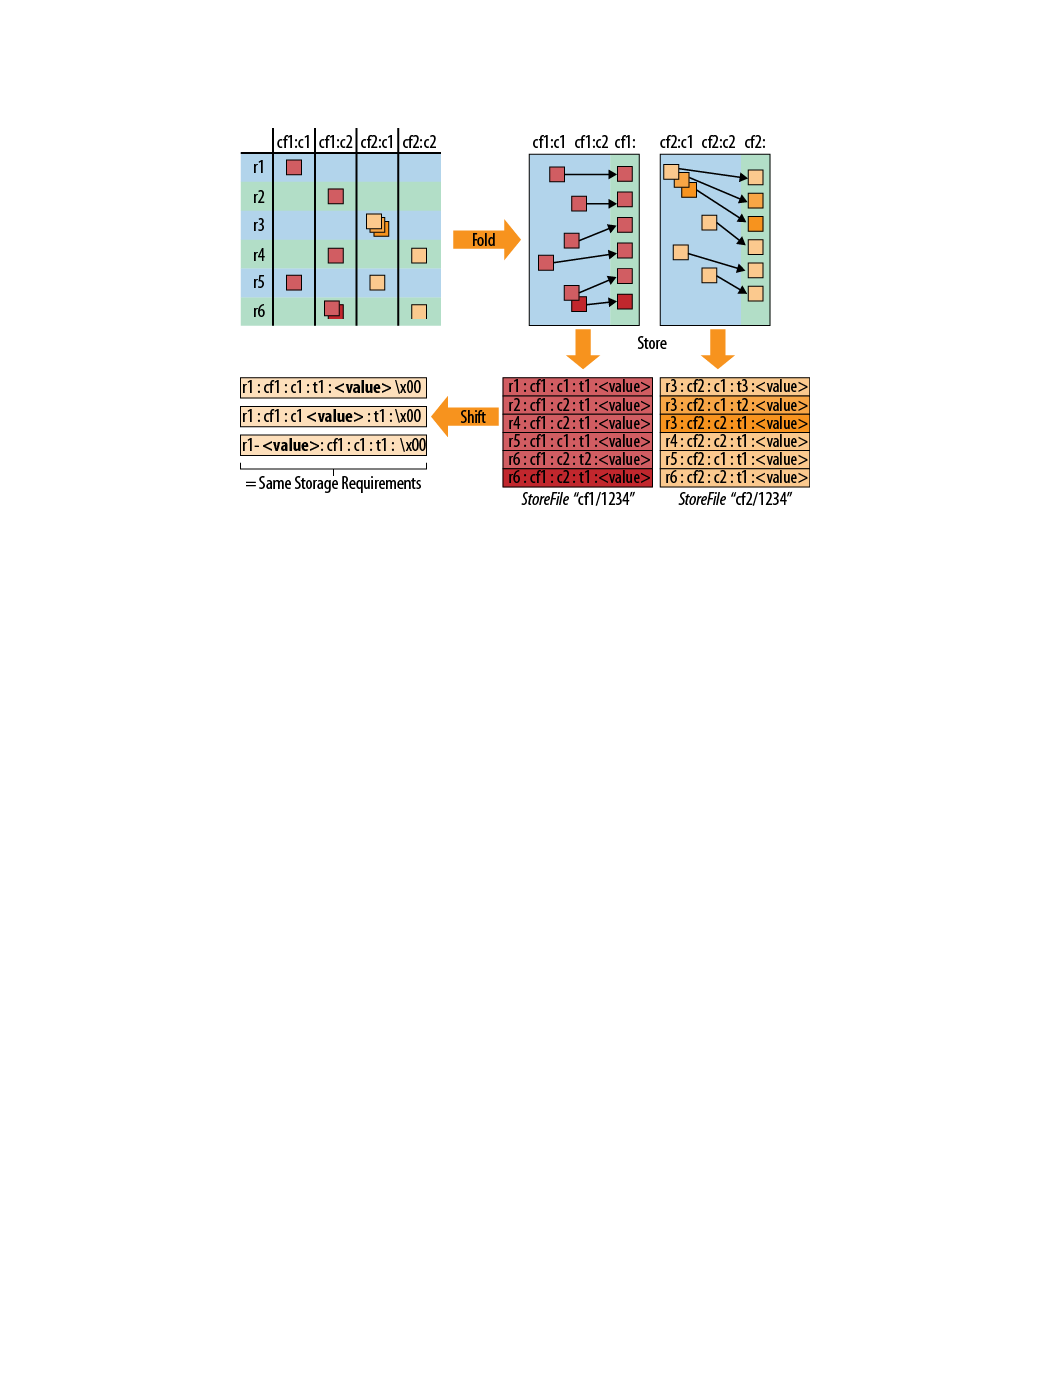
\includegraphics[scale=0.7]{./figures/layout}
  \end{figure}

  \begin{itemize}
  \item \textbf{Physical Layout (Lower-Right)}
    \begin{itemize}
    \item Select data by row key
      \begin{itemize}
      \item This reduces the amount of data to scan for a row or a
        range of rows
      \end{itemize}
    \item Select data by row key and column key
      \begin{itemize}
      \item This focuses the system on an individual storage file
      \end{itemize}
    \item Select data by column qualifier
      \begin{itemize}
      \item Exact lookups, including filters to omit useless data
      \end{itemize}
    \end{itemize}
  \end{itemize}
}

\frame {\frametitle{Concepts}
  \begin{itemize}
  \item \textbf{Summary of key lookup properties}
  \end{itemize}

\vspace{20pt}

 \begin{figure}[h]
    \centering
    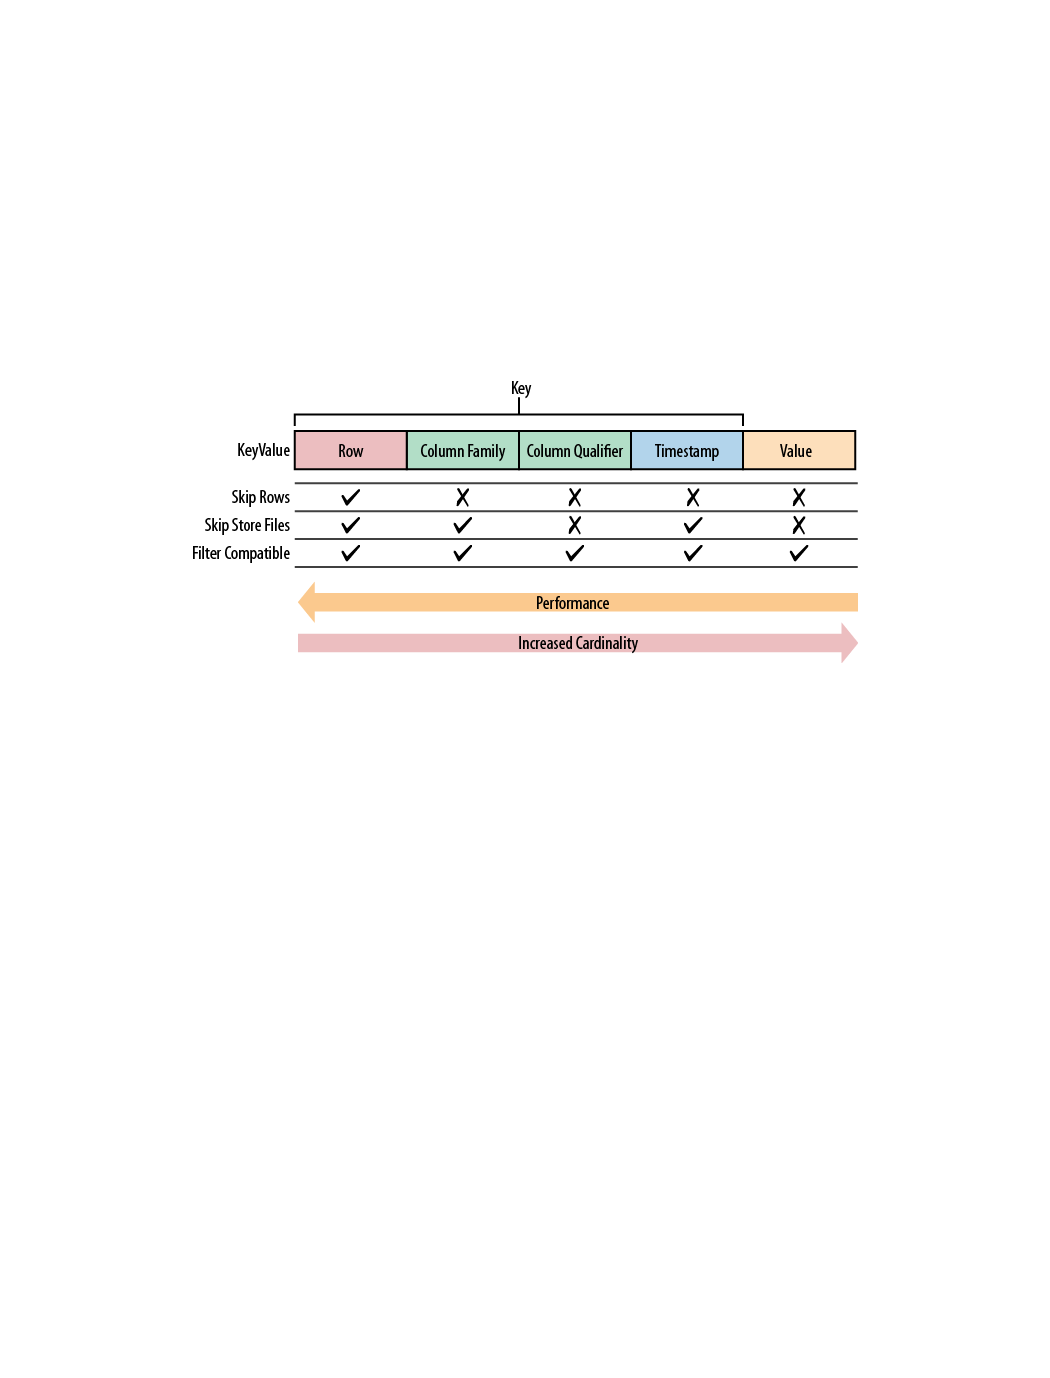
\includegraphics[scale=0.8]{./figures/key-lookup}
  \end{figure}

}

%%%%%%%%%%%%%%%%%%%%%%%%%%%%%%%%%%%%%%%%%%%%%%%%%%%%%%%%%%
\subsection{Tall-Narrow vs. Flat-Wide}
%%%%%%%%%%%%%%%%%%%%%%%%%%%%%%%%%%%%%%%%%%%%%%%%%%%%%%%%%%
\frame {\frametitle{Tall-Narrow vs. Flat-Wide Tables}
  \begin{itemize}
  \item \textbf{Tall-Narrow Tables}
    \begin{itemize}
    \item Few columns
    \item Many rows
    \end{itemize}

    \vspace{20pt}

  \item \textbf{Flat-Wide Tables}
    \begin{itemize}
    \item Many columns
    \item Few rows
    \end{itemize}

    \vspace{20pt}

  \item \textbf{Given the query granularity explained before}
    \begin{itemize}
    \item[$\to$] Store parts of the cell data in the row key
    \item Furthermore, HBase splits at row boundaries
    \item[$\to$] It is recommended to go for Tall-Narrow Tables
    \end{itemize}

  \end{itemize}
}

\frame {\frametitle{Tall-Narrow vs. Flat-Wide Tables}
  \begin{itemize}
  \item \textbf{Example: email data - version 1}
    \begin{itemize}
    \item You have all emails of a user in a single row (e.g. \texttt{userID}
      is the row key)
    \item There will be some outliers with orders of magnitude more
      emails than others
    \item[$\to$] A single row could outgrow the maximum file/region
      size and work against split facility
    \end{itemize}

    \vspace{20pt}

  \item \textbf{Example: email data - version 2}
    \begin{itemize}
    \item Each email of a user is stored in a separate row
      (e.g. \texttt{userID:messageID} is the row key)
    \item On disk this makes no difference (see the disk layout
      figure)
      \begin{itemize}
      \item If the \texttt{messageID} is in the column qualifier or
        the row key, each cell still contains a single email message
      \end{itemize}
    \item[$\to$] The table can be split easily and the query
      granularity is more fine-grained
    \end{itemize}

  \end{itemize}

}


%%%%%%%%%%%%%%%%%%%%%%%%%%%%%%%%%%%%%%%%%%%%%%%%%%%%%%%%%%
\subsection{Partial Key Scans}
%%%%%%%%%%%%%%%%%%%%%%%%%%%%%%%%%%%%%%%%%%%%%%%%%%%%%%%%%%
\frame {\frametitle{Partial Key Scans}
  \begin{itemize}
  \item \textbf{Partial Key Scans reinforce the concept of Tall-Narrow Tables}
    \begin{itemize}
    \item From the email example: assume you have a separate row per
      message, across all users
    \item If you don't have an exact combination of user and message
      ID you cannot access a particular message
    \end{itemize}

    \vspace{20pt}

  \item \textbf{Partial Key Scan solves the problems}
    \begin{itemize}
    \item Specify a \textit{start} and \textit{end} key
    \item The start key is set to the exact \texttt{userID} only, with the
      end key set at \texttt{userID+1}
    \item[$\to$] This triggers the internal lexicographic comparison
      mechanism
      \begin{itemize}
      \item Since the table does not have an exact match, it positions
        the scan at: \texttt{<userID>:<lowest-messageID>}
      \end{itemize}
    \item The scan will then iterate over all the messages of an exact
      user, parse the row key and get the \texttt{messageID}
    \end{itemize}

  \end{itemize}
}

\frame {\frametitle{Partial Key Scans}
  \begin{itemize}
  \item \textbf{Composite keys and atomicity}
    \begin{itemize}
    \item Following the email example: a single user inbox now spans
      many rows
    \item It is no longer possible to modify a single user inbox in
      one atomic operation
    \end{itemize}

    \vspace{20pt}

  \item \textbf{If this is acceptable or not, depends on the application at hand}

  \end{itemize}
}

%%%%%%%%%%%%%%%%%%%%%%%%%%%%%%%%%%%%%%%%%%%%%%%%%%%%%%%%%%
\subsection{Time Series Data}
%%%%%%%%%%%%%%%%%%%%%%%%%%%%%%%%%%%%%%%%%%%%%%%%%%%%%%%%%%
\frame {\frametitle{Time Series Data}
  \begin{itemize}
  \item \textbf{Stream processing of events}
    \begin{itemize}
    \item E.g. data coming from a sensor, stock exchange, monitoring
      system ...
    \item Such data is a time series $\to$ \textbf{The row key represents the
      event time}
  \item[$\to$] HBase will store all rows sorted in a distinct range,
    namely regions with specific start and stop keys
    \end{itemize}

    \vspace{20pt}

  \item \textbf{Sequential monotonously increasing nature of time
      series data}
    \begin{itemize}
    \item All incoming data is written to the same region (and hence
      the same server)
    \item[$\to$] \textbf{Regions become HOT!}
    \item Performance of the whole cluster is bound to that of a
      single machine
    \end{itemize}
  \end{itemize}
}

\frame {\frametitle{Time Series Data}
  \begin{itemize}
  \item \textbf{Solution to achieve load balancing: Salting}
    \begin{itemize}
    \item We want data to be spread over all region servers
    \item This can be done, e.g., by prefixing the row key with a
      non-sequential number
    \end{itemize}
  \end{itemize}
  
  \vspace{10pt}
  
  \begin{beamerboxesrounded}{\textbf{Salting example}}
    
    \begin{footnotesize}
      \texttt{byte prefix = (byte) (Long.hashCode(timestamp) \% <number of region servers>);\\
        byte[] rowkey = Bytes.add(Bytes.toBytes(prefix),
        Bytes.toBytes(timestamp));}
    \end{footnotesize} 
  \end{beamerboxesrounded}

  \vspace{10pt}

  \begin{itemize}
  \item[\textbf{-}]Data access needs to be \textit{fanned out} across many
    servers
  \item[\textbf{+}] Use multiple threads to read for I/O performance: e.g. use the Map
    phase of MapReduce 
  \end{itemize}  
}

\frame {\frametitle{Time Series Data}
  \begin{itemize}
  \item \textbf{Solution to achieve load balancing: Field swap/promotion}
    \begin{itemize}
    \item Move the timestamp filed of the row key or prefix it with
      another field
      \begin{itemize}
      \item If you already have a composite row key, simply \textit{swap}
        elements
      \item Otherwise if you only have the timestamp, you need to
        \textit{promote} another field
      \end{itemize}
    \item The sequential, monotonously increasing timestamp is moved
      to a secondary position in the row key
    \end{itemize}
    
    \vspace{20pt}
    
  \item[\textbf{-}] You can only access data (especially time ranges)
    for a given swapped or promoted field (but this could be a feature)
  \item[\textbf{+}] You achieve load balancing 
  \end{itemize}
}

\frame {\frametitle{Time Series Data}
  \begin{itemize}
  \item \textbf{Solution to achieve load balancing: Randomization}
    \begin{itemize}
    \item \texttt{byte[] rowkey = MD5(timestamp)}
    \item This gives you a random distribution of the row key across
      all available region servers
    \end{itemize}

    \vspace{20pt}

  \item[\textbf{-}] Less than ideal for range scans
  \item[\textbf{+}] Since you can re-hash the timestamp, this solution
    is good for \textbf{random access}
  \end{itemize}
}

\frame {\frametitle{Time Series Data}
  \begin{itemize}
  \item \textbf{Summary}
  \end{itemize}

  \begin{figure}[h]
    \centering
    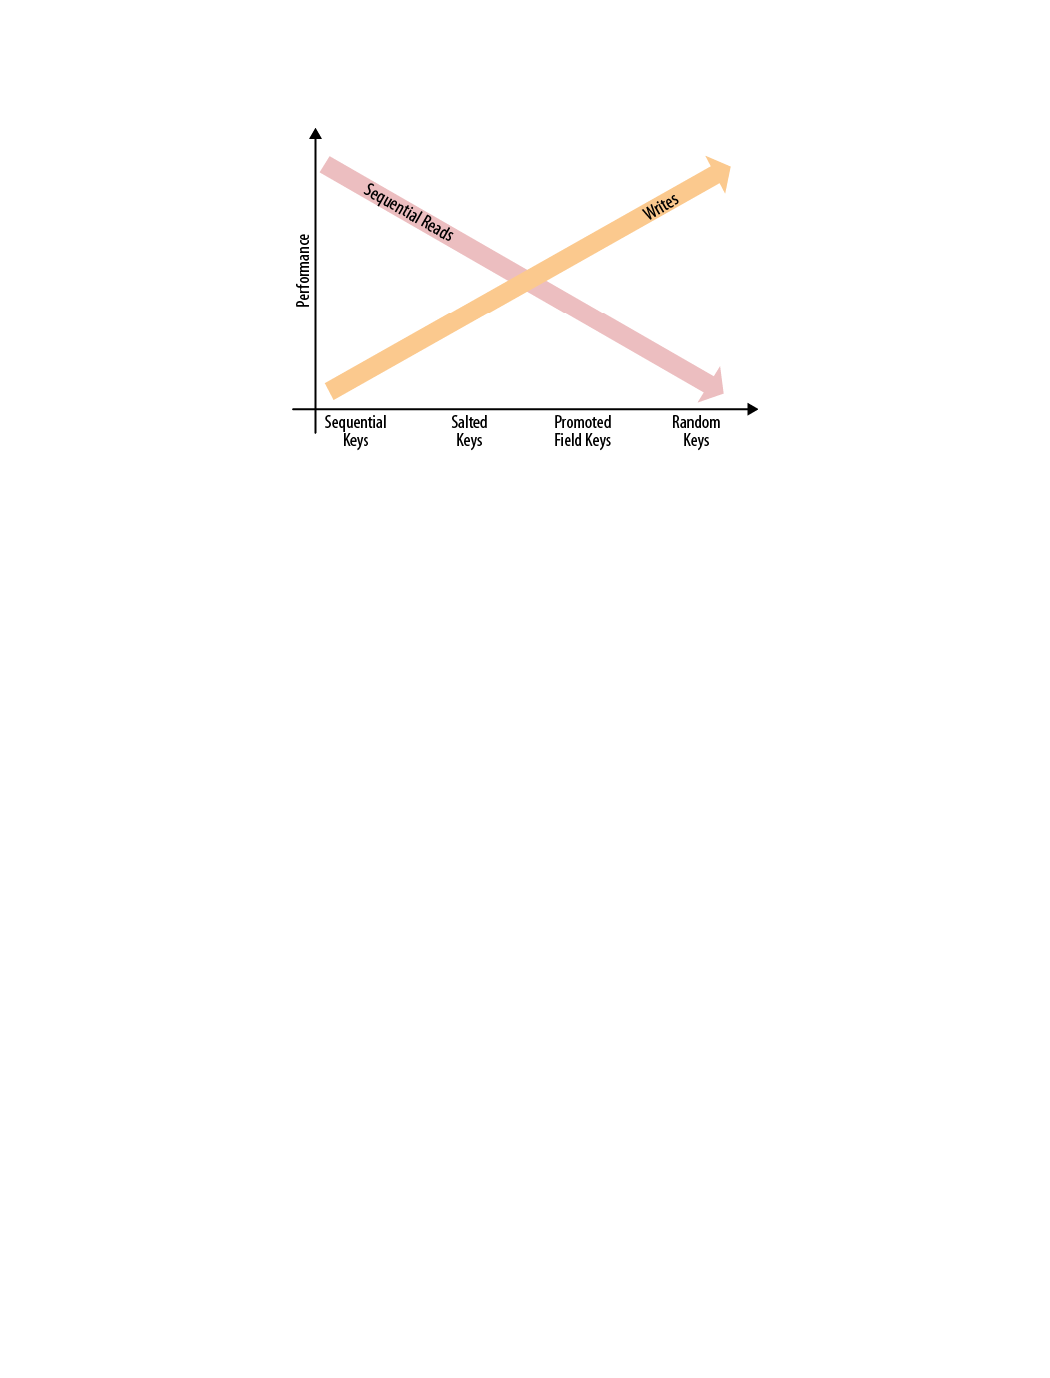
\includegraphics[scale=0.8]{./figures/time-series}
  \end{figure}

}

% %%%%%%%%%%%%%%%%%%%%%%%%%%%%%%%%%%%%%%%%%%%%%%%%%%%%%%%%%%
% \subsection{Time-Ordered Relations}
% %%%%%%%%%%%%%%%%%%%%%%%%%%%%%%%%%%%%%%%%%%%%%%%%%%%%%%%%%%
% \frame {\frametitle{}
% }

